%!TEX TS-program = pdflatex
%!TEX TS-options = -shell-escape
% ============================================================
%  Einführung in die Programmiersprache C
%  Vorlesung Embedded Systems Engineering
%  Prof. Dr.-Ing. Sebastian Schlesinger
%  HWR Berlin, Wintersemester 2026
% ============================================================

% xcolor muss vor beamer mit Optionen gepatcht werden
\PassOptionsToPackage{usenames,x11names}{xcolor}

\documentclass[%
  aspectratio=169,
  10pt
]{beamer}

% -----------------------------------------------------------
%  Sprache und Encoding
% -----------------------------------------------------------
\usepackage[utf8]{inputenc}
\usepackage[T1]{fontenc}
% Umlaute funktionieren über inputenc/fontenc ohne babel.
% Deutsche Anführungszeichen (ohne babel-german)
\usepackage{textcomp}
\newcommand{\enquote}[1]{\quotedblbase{}#1\textquotedblleft{}}

% -----------------------------------------------------------
%  Fonts
% -----------------------------------------------------------
\usepackage{charter}
\usepackage{courier}                % Monospace-Font für Listings
\renewcommand{\ttdefault}{pcr}      % Courier als tt-Font
% microtype: nur protrusion, kein font-expansion (Beamer-kompatibel)
\usepackage[protrusion=true,expansion=false]{microtype}

% -----------------------------------------------------------
%  Farben  (wie config.tex der Übungsblätter)
% -----------------------------------------------------------
\definecolor{fbblau}{HTML}{3078AB}
\definecolor{blackberry}{rgb}{0.53, 0.0, 0.25}
\definecolor{codebg}{rgb}{0.97, 0.97, 0.97}

% -----------------------------------------------------------
%  Beamer-Theme (angepasst an ESE-Stil)
% -----------------------------------------------------------
\usetheme{default}
\useinnertheme{rectangles}

%  Strukturfarbe
\setbeamercolor{structure}{fg=fbblau}

%  Titelfolie
\setbeamercolor{title}{fg=white, bg=fbblau}
\setbeamercolor{subtitle}{fg=fbblau!25!white, bg=fbblau}
\setbeamercolor{author}{fg=white, bg=fbblau}
\setbeamercolor{institute}{fg=fbblau!20!white, bg=fbblau}
\setbeamercolor{date}{fg=fbblau!20!white, bg=fbblau}

%  Folienrahmen
\setbeamercolor{frametitle}{fg=white, bg=fbblau}
\setbeamerfont{frametitle}{series=\bfseries, size=\normalsize}

%  Inhaltsverzeichnis
\setbeamercolor{section in toc}{fg=fbblau}
\setbeamerfont{section in toc}{series=\bfseries}

%  Blöcke
\setbeamercolor{block title}{bg=fbblau, fg=white}
\setbeamercolor{block body}{bg=fbblau!8, fg=black}
\setbeamercolor{alertblock title}{bg=blackberry, fg=white}
\setbeamercolor{alertblock body}{bg=blackberry!8, fg=black}
\setbeamercolor{exampleblock title}{bg=fbblau!70!black, fg=white}
\setbeamercolor{exampleblock body}{bg=fbblau!6, fg=black}

%  Aufzählungspunkte
\setbeamercolor{item}{fg=fbblau}
\setbeamercolor{subitem}{fg=fbblau!70}
\setbeamertemplate{itemize item}{\small$\triangleright$}
\setbeamertemplate{itemize subitem}{\small$\triangleright$}

%  Navigationsleiste ausblenden
\setbeamertemplate{navigation symbols}{}

%  Fußzeile
\setbeamertemplate{footline}{%
  \leavevmode
  \hbox{%
    \begin{beamercolorbox}[wd=.50\paperwidth,ht=2.25ex,dp=1ex,
                           left,leftskip=2mm]{palette primary}%
      \usebeamerfont{author in head/foot}%
      \textbf{ESE} \,|\, Einführung in C \,|\, \insertshortauthor
    \end{beamercolorbox}%
    \begin{beamercolorbox}[wd=.40\paperwidth,ht=2.25ex,dp=1ex,
                           center]{palette secondary}%
      \usebeamerfont{title in head/foot}\insertsection
    \end{beamercolorbox}%
    \begin{beamercolorbox}[wd=.10\paperwidth,ht=2.25ex,dp=1ex,
                           right,rightskip=2mm]{palette primary}%
      \insertframenumber\,/\,\inserttotalframenumber
    \end{beamercolorbox}%
  }%
}

%  Sectiontrenner
\AtBeginSection[]{%
  \begin{frame}[plain]
    \vfill
    \centering
    \begin{beamercolorbox}[sep=12pt,center,shadow=false,rounded=false,
                           wd=0.8\textwidth]{title}
      \usebeamerfont{title}\insertsectionhead
    \end{beamercolorbox}
    \vfill
  \end{frame}
}

% -----------------------------------------------------------
%  Code-Listings  (wie config.tex)
% -----------------------------------------------------------
\usepackage{listings}
\lstset{%
  language        = C,
  basicstyle      = \ttfamily\footnotesize,
  keywordstyle    = \color{fbblau}\bfseries,
  commentstyle    = \color{gray}\itshape,
  stringstyle     = \color{blackberry},
  numberstyle     = \tiny\color{gray},
  numbers         = left,
  numbersep       = 8pt,
  stepnumber      = 1,
  frame           = single,
  framesep        = 3pt,
  rulecolor       = \color{fbblau!40},
  backgroundcolor = \color{codebg},
  showstringspaces= false,
  breaklines      = true,
  columns         = fullflexible,
  keepspaces      = true,
  xleftmargin     = 1.2em,
  xrightmargin    = 0.3em,
  tabsize         = 4,
  morekeywords    = {uint8_t,uint16_t,uint32_t,uint64_t,
                     int8_t,int16_t,int32_t,int64_t,
                     bool,true,false,NULL,size_t,ptrdiff_t,
                     volatile,inline,restrict,_Bool,
                     va_list,va_start,va_arg,va_end},
  % Umlaute in lstlisting-Umgebungen ermöglichen
  literate        = {ä}{{\"a}}1 {ö}{{\"o}}1 {ü}{{\"u}}1
                    {Ä}{{\"A}}1 {Ö}{{\"O}}1 {Ü}{{\"U}}1
                    {ß}{{\ss}}1
}

% -----------------------------------------------------------
%  Weitere Pakete
% -----------------------------------------------------------
\usepackage{tikz}
\usetikzlibrary{arrows.meta, shapes, positioning, calc, matrix}
\usepackage{booktabs}
\usepackage{array}
\usepackage{multicol}

% -----------------------------------------------------------
%  Metadaten
% -----------------------------------------------------------
\title[Einführung in C]{Einführung in die Programmiersprache C}
\subtitle{Embedded Systems Engineering -- Vorlesung}
\author[Schlesinger]{Prof.\,Dr.\,-Ing.\ Sebastian Schlesinger}
\institute{%
  Fachbereich 2 -- Duales Studium Wirtschaft \& Technik\\
  HWR Berlin}
\date{Wintersemester 2026}

% ============================================================
\begin{document}
% ============================================================

% -----------------------------------------------------------
%  TITELFOLIE
% -----------------------------------------------------------
\begin{frame}[plain]
  \titlepage
\end{frame}

% -----------------------------------------------------------
%  GLIEDERUNG
% -----------------------------------------------------------
\begin{frame}{Gliederung}
  \tableofcontents
\end{frame}

% ============================================================
\section{Geschichte und Entwicklung von C}
% ============================================================

\begin{frame}{Ursprünge: Von BCPL zu C}
  \begin{columns}[T]
    \begin{column}{0.58\textwidth}
      \textbf{Die Entwicklungslinie:}
      \begin{itemize}
        \item \textbf{1967} -- Martin Richards: \textbf{BCPL}
              (\emph{Basic Combined Programming Language}),\\
              typlos, für Systemprogrammierung
        \item \textbf{1969} -- Ken Thompson: \textbf{B} bei Bell Labs,\\
              vereinfachtes BCPL für die PDP-7
        \item \textbf{1972} -- Dennis Ritchie: \textbf{C} -- direkt gekoppelt\\
              an die Reimplementierung von \textbf{Unix} auf der PDP-11
        \item \textbf{1978} -- \emph{The C Programming Language},\\
              Kernighan \& Ritchie (\enquote{K\&R}) -- informeller Standard
      \end{itemize}
    \end{column}
    \begin{column}{0.38\textwidth}
      \begin{block}{Schlüsselpersonen}
        \textbf{Dennis M. Ritchie} (1941--2011)\\
        Schöpfer von C, Miterfinder von Unix\\[0.3em]
        \textbf{Ken Thompson} (*1943)\\
        Miterfinder von Unix und B\\[0.3em]
        \textbf{Brian W. Kernighan} (*1942)\\
        Co-Autor von K\&R C
      \end{block}
      \begin{alertblock}{Zitat Ritchie}
        \emph{„C is quirky, flawed, and an enormous success."}
      \end{alertblock}
    \end{column}
  \end{columns}

  \vspace{0.4em}
  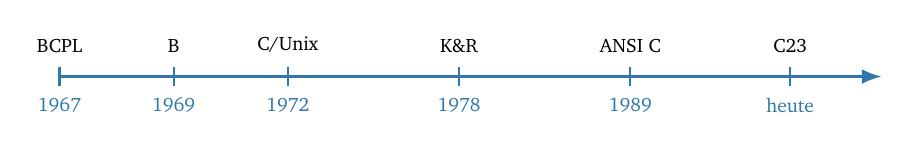
\begin{tikzpicture}[x=1.45cm]
    \draw[-{Latex[length=2.5mm]}, thick, fbblau] (0,0) -- (7.2,0);
    \foreach \pos/\lab/\desc in {%
      0/{1967}/{BCPL},
      1/{1969}/{B},
      2/{1972}/{C/Unix},
      3.5/{1978}/{K\&R},
      5/{1989}/{ANSI C},
      6.4/{heute}/{C23}}{%
      \draw[fbblau, thick] (\pos, 0.12) -- (\pos, -0.12);
      \node[below, fbblau, font=\scriptsize] at (\pos, -0.15) {\lab};
      \node[above, font=\scriptsize]         at (\pos,  0.18) {\desc};
    }
  \end{tikzpicture}
\end{frame}

\begin{frame}{Die C-Standards im Überblick}
  \begin{block}{}
    \small
    \begin{tabular}{>{\bfseries}l l p{8cm}}
      \toprule
      Standard      & Jahr  & Wichtigste Neuerungen \\
      \midrule
      K\&R C        & 1978  & Ursprüngliche informelle Definition \\
      ANSI C / C89  & 1989  & Erster ISO-Standard (ISO/IEC 9899:1990) \\
      C95           & 1995  & Trigraphs, \texttt{wchar.h}, Erweiterungen \\
      \textcolor{fbblau}{\textbf{C99}} & \textcolor{fbblau}{\textbf{1999}}
                             & \texttt{//}-Kommentare, \texttt{bool}, VLAs, \texttt{stdint.h},
                               gemischte Deklarationen, \texttt{inline} \\
      C11           & 2011  & \texttt{\_Atomic}, \texttt{<threads.h>}, \texttt{\_Generic},
                               anonyme Structs \\
      C17 / C18     & 2018  & Bugfixes, keine neuen Features \\
      \textcolor{fbblau}{\textbf{C23}} & \textcolor{fbblau}{\textbf{2023}}
                             & \texttt{nullptr}, \texttt{bool} als Keyword, \texttt{\#embed},
                               \texttt{typeof}, Attribute \\
      \bottomrule
    \end{tabular}
  \end{block}

  \vspace{0.3em}
  \begin{columns}[T]
    \begin{column}{0.48\textwidth}
      \textbf{Relevanz für Embedded Systems:}
      \begin{itemize}
        \item Toolchains (GCC ARM, IAR, Keil) unterstützen primär \textbf{C99} und \textbf{C11}
        \item MISRA-C (2012, 2023) schreibt ein sicheres Subset vor
        %\item Portabilität erfordert Kenntnis des eingesetzten Standards
      \end{itemize}
    \end{column}
    \begin{column}{0.48\textwidth}
      \begin{alertblock}{Kompilierung mit Standard}
        \texttt{gcc -std=c11 -Wall -Wextra -o prog prog.c}\\[0.2em]
        Immer den Standard explizit angeben -- der Compiler-Default
        kann sich zwischen Versionen ändern!
      \end{alertblock}
    \end{column}
  \end{columns}
\end{frame}

\begin{frame}{Warum C für Embedded Systems?}
  \begin{columns}[T]
    \begin{column}{0.48\textwidth}
      \textbf{Stärken:}
      \begin{itemize}
        \item \textbf{Hardwarenähe:} direkte Speicher- und
              Registerzugriffe über Pointer
        \item \textbf{Effizienz:} minimaler Laufzeit-Overhead,
              kein Garbage Collector
        \item \textbf{Deterministismus:} kein JIT, vorhersagbares
              Timing -- kritisch für Echtzeitsysteme
        \item \textbf{Portabilität:} läuft auf nahezu jeder
              Prozessorarchitektur (ARM, RISC-V, AVR, MSP430 \ldots)
        \item \textbf{Reife Toolchain:} GCC, Clang, LLVM, IAR,
              MISRA-Checker, statische Analysetools
      \end{itemize}
    \end{column}
    \begin{column}{0.48\textwidth}
      \textbf{Herausforderungen:}
      \begin{itemize}
        \item Kein automatisches Speichermanagement
        \item Fehleranfällig: Buffer Overflows, Dangling Pointers,
              undefined Behavior
        \item Kein eingebautes OOP, kein Exception Handling
        \item Kein nativer Modulmechanismus (nur \texttt{\#include})
      \end{itemize}
      \vspace{0.4em}
      \begin{alertblock}{Leitsatz}
        C gibt dem Programmierer \emph{alle} Freiheiten -- \\
        und damit \emph{alle} Verantwortung.
      \end{alertblock}
    \end{column}
  \end{columns}
\end{frame}

% ============================================================
\section{Grundkonstrukte}
% ============================================================

\begin{frame}[fragile]{Struktur eines C-Programms}
  \begin{columns}[T]
    \begin{column}{0.52\textwidth}
\begin{lstlisting}
/* Präprozessor-Direktiven */
#include <stdio.h>     /* I/O Standardbibliothek */
#include <stdint.h>    /* Exakte Integer-Typen   */
#define MAX_SIZE  128  /* Makro (keine Variable!) */
/* Globale Variable (Filescope) */
static int counter = 0;
/* Funktionsprototyp (Deklaration) */
void print_hello(const char *msg);

/* Hauptprogramm */
int main(void) {
    print_hello("Hello, ESE!");
    return 0;  /* 0 = Erfolg, != 0 = Fehler */
}
/* Funktionsdefinition */
void print_hello(const char *msg) {
    printf("%s\n", msg);
}
\end{lstlisting}
    \end{column}
    \begin{column}{0.45\textwidth}
      \textbf{Übersetzungsprozess:}
      \begin{enumerate}
        \item \textbf{Präprozessor} (\texttt{cpp}):
              \texttt{\#include}, \texttt{\#define}, bedingte
              Kompilierung
        \item \textbf{Compiler} (\texttt{cc1}):
              C $\rightarrow$ Assembler (\texttt{.s})
        \item \textbf{Assembler} (\texttt{as}):
              Assembler $\rightarrow$ Objektcode (\texttt{.o})
        \item \textbf{Linker} (\texttt{ld}):
              \texttt{.o} + Libs $\rightarrow$ Executable
      \end{enumerate}
      \vspace{0.3em}
      \begin{block}{Wichtige Compiler-Flags}
        \texttt{-Wall -Wextra} -- alle Warnungen\\
        \texttt{-O2} -- Optimierung\\
        \texttt{-g} -- Debug-Info\\
        \texttt{-std=c11} -- C-Standard
      \end{block}
    \end{column}
  \end{columns}
\end{frame}

\begin{frame}[fragile]{Primitive Datentypen}
  \begin{columns}[T]
    \begin{column}{0.48\textwidth}
      \begin{block}{Ganzzahl-Typen (plattformabhängig!)}
        \small
        \begin{tabular}{l l l}
          \texttt{char}       & 1\,Byte  & $-128 \ldots 127$ \\
          \texttt{short}      & 2\,Byte  & $\pm 32\,767$ \\
          \texttt{int}        & 2--4\,B* & \\
          \texttt{long}       & 4--8\,B* & \\
          \texttt{long long}  & 8\,Byte  & $\pm 9{,}2 \cdot 10^{18}$
        \end{tabular}\\[0.3em]
        \footnotesize{*Größe plattformabhängig!}
      \end{block}
      \begin{exampleblock}{Portable Typen -- \texttt{<stdint.h>} (C99)}
        \texttt{int8\_t},  \texttt{uint8\_t}   -- 8\,Bit\\
        \texttt{int16\_t}, \texttt{uint16\_t}  -- 16\,Bit\\
        \texttt{int32\_t}, \texttt{uint32\_t}  -- 32\,Bit\\
        \texttt{int64\_t}, \texttt{uint64\_t}  -- 64\,Bit
      \end{exampleblock}
    \end{column}
    \begin{column}{0.48\textwidth}
      \begin{block}{Gleitkomma- und sonstige Typen}
        \texttt{float}   -- 4\,Byte, $\approx$7 Dezimalstellen\\
        \texttt{double}  -- 8\,Byte, $\approx$15 Stellen\\
        \texttt{void}    -- kein Typ\\
        \texttt{bool} / \texttt{\_Bool}  -- wahr/falsch (C99)
      \end{block}
\begin{lstlisting}
#include <stdint.h>
#include <stdbool.h>

uint8_t  reg   = 0xFF;    /* 8-Bit Register */
int32_t  count = -1;
float    volt  = 3.3f;    /* f: float-Literal */
double   pi    = 3.14159265358979;
char     c     = 'A';     /* = 65 = 0x41  */
bool     flag  = true;
\end{lstlisting}
      \begin{alertblock}{Embedded-Regel}
        Immer \texttt{stdint.h}-Typen verwenden --\\
        niemals auf \texttt{int}-Größe verlassen!
      \end{alertblock}
    \end{column}
  \end{columns}
\end{frame}

\begin{frame}[fragile]{Operatoren}
  \begin{columns}[T]
    \begin{column}{0.32\textwidth}
      \textbf{Arithmetisch:}
\begin{lstlisting}
int a = 10, b = 3;
a + b   /* 13 */
a - b   /* 7  */
a * b   /* 30 */
a / b   /* 3 (int!) */
a % b   /* 1 (Modulo)*/
\end{lstlisting}
      \textbf{Vergleich / Logik:}
\begin{lstlisting}
a == b  /* falsch: 0 */
a != b  /* wahr: 1  */
a > b   /* 1        */
a && b  /* logisch  */
a || b
!a
\end{lstlisting}
    \end{column}
    \begin{column}{0.34\textwidth}
      \textbf{Bitweise (für Embedded!):}
\begin{lstlisting}
uint8_t r = 0b10110100;

r & 0x0F   /* AND:  0x04  */
r | 0x01   /* OR:   0xB5  */
r ^ 0xFF   /* XOR:  0x4B  */
~r         /* NOT:  0x4B  */
r << 2     /* Links shift */
r >> 1     /* Rechts shift*/
/* Bit setzen */
r |= (1u << 3);
/* Bit löschen */
r &= ~(1u << 3);
/* Bit testen */
if (r & (1u << 3)) { }
\end{lstlisting}
    \end{column}
    \begin{column}{0.30\textwidth}
      \textbf{Zuweisung und Sonstiges:}
\begin{lstlisting}
a += 5;  a -= 5;
a *= 2;  a /= 2;
a &= 0xF0;
a |= 0x01;
a++;   /* Postfix */
++a;   /* Präfix  */
a--;
/* Ternär: */
int m = (a>b)?a:b;

/* sizeof */
sizeof(int32_t) /* 4 */
sizeof(arr)/
  sizeof(arr[0])/* Anz. Elemente */
\end{lstlisting}
      % \begin{alertblock}{Achtung}
      %   Integer Division: \texttt{5/2 == 2}!
      % \end{alertblock}
    \end{column}
  \end{columns}
\end{frame}

\begin{frame}[fragile]{Kontrollstrukturen}
  \begin{columns}[T]
    \begin{column}{0.47\textwidth}
      \textbf{Bedingte Ausführung:}
\begin{lstlisting}
if (voltage > 3.0f) {
    set_led(GREEN);
} else if (voltage > 2.0f) {
    set_led(YELLOW);
} else {
    set_led(RED);
    shutdown();
}
/* Switch für Zustandsmaschinen */
switch (state) {
  case STATE_IDLE:
    handle_idle();   break;
  case STATE_RUN:
    handle_run();    break;
  case STATE_ERROR:
    handle_error();  break;
  default:
    /* sollte nie eintreten */
    assert(false);   break;
}
\end{lstlisting}
    \end{column}
    \begin{column}{0.50\textwidth}
      \textbf{Schleifen:}
\begin{lstlisting}
/* For-Schleife (Zählschleife) */
for (uint32_t i = 0; i < N; i++) {
    buffer[i] = 0u;
}
/* While (kopfgesteuert) */
while (!uart_tx_ready()) {
    /* warte auf Hardware */
}
/* Do-While (mindestens einmal) */
uint16_t sample;
do {
    sample = adc_read();
} while (sample < THRESHOLD);
/* break / continue */
for (int i = 0; i < 100; i++) {
    if (i == 50) break;   /* Abbruch */
    if (i % 2)  continue; /* Sprung  */
    process(i);
}
\end{lstlisting}
    \end{column}
  \end{columns}
\end{frame}

\begin{frame}[fragile]{Funktionen und Speicherklassen}
  \begin{columns}[T]
    \begin{column}{0.50\textwidth}
\begin{lstlisting}
/* Deklaration (Header) */
int32_t clamp(int32_t val,
              int32_t lo, int32_t hi);
/* Definition */
int32_t clamp(int32_t val,
              int32_t lo, int32_t hi) {
    if (val < lo) return lo;
    if (val > hi) return hi;
    return val;
}
/* Rekursion */
uint64_t factorial(uint32_t n) {
    return (n <= 1u) ? 1u
                     : n * factorial(n-1u);
}
/* Statische lokale Variable */
uint32_t next_id(void) {
    static uint32_t id = 0u;
    return ++id;   /* persistiert! */
}
\end{lstlisting}
    \end{column}
    \begin{column}{0.47\textwidth}
      \textbf{Speicherklassen und Qualifier:}
      \begin{itemize}
        \item \texttt{auto} -- lokal, Stack (Standard)
        \item \texttt{static} -- persistiert / Filescope
        \item \texttt{extern} -- externe Bindung
        \item \texttt{inline} -- Compiler-Inlining-Hint
        \item \texttt{volatile} -- externe Manipulation möglich; keine Compiler-Optimierung
      \end{itemize}
      \vspace{0.3em}
      \begin{alertblock}{\texttt{volatile} -- wichtig in Embedded!}
\begin{lstlisting}
/* Ohne volatile: Compiler könnte
   Schleife wegoptimieren!       */
volatile uint32_t *timer_reg =
    (volatile uint32_t*)0x40001000;

while (*timer_reg < 1000u) {
    ; /* warte */
}
\end{lstlisting}
        %\small Verwenden bei: Hardware-Registern,
        %ISR-Flags, Shared Memory in RTOS-Systemen
      \end{alertblock}
    \end{column}
  \end{columns}
\end{frame}

\begin{frame}[fragile]{Arrays, Strings und zusammengesetzte Typen}
  \begin{columns}[T]
    \begin{column}{0.48\textwidth}
      \textbf{Arrays:}
\begin{lstlisting}
uint8_t buf[8]   = {0};      /* 0-initialisiert */
int     fib[]    = {1,1,2,3,5,8}; /* Größe auto */
int     mat[3][3]= {{1,0,0},
                    {0,1,0},
                    {0,0,1}};
/* Größe zur Laufzeit (C99 VLA) */
void fill(size_t n, int arr[n]);
\end{lstlisting}
      \textbf{Strings (Null-terminierte char-Arrays):}
\begin{lstlisting}
char name[] = "ESE";  /* {'E','S','E','\0'} */
char buf[32];

/* Sichere Funktionen (string.h) */
strncpy(buf, name, sizeof(buf)-1);
buf[sizeof(buf)-1] = '\0';  /* sicher! */
size_t len = strlen(name);  /* 3 */
\end{lstlisting}
    \end{column}
    \begin{column}{0.48\textwidth}
      \textbf{Struct und Enum:}
\begin{lstlisting}
typedef enum {
    STATE_IDLE = 0,
    STATE_RUNNING,
    STATE_ERROR
} State_t;

typedef struct {
    uint32_t  id;
    float     temperature;
    State_t   state;
} Sensor_t;

/* Designated Initializer (C99) */
Sensor_t s = {
    .id          = 1u,
    .temperature = 23.5f,
    .state       = STATE_IDLE
};

printf("T=%.1f\n", s.temperature);
s.state = STATE_RUNNING;
\end{lstlisting}
    \end{column}
  \end{columns}
\end{frame}

% ============================================================
\section{Zeiger (Pointer)}
% ============================================================

\begin{frame}[fragile]{Grundlagen: Was ist ein Pointer?}
  \begin{columns}[T]
    \begin{column}{0.52\textwidth}
\begin{lstlisting}
int  x = 42;
int *p = &x;   /* p enthält Adresse von x */
printf("Wert x:    %d\n",  x);   /* 42   */
printf("Adresse x: %p\n", &x);   /* 0x.. */
printf("Pointer p: %p\n",  p);   /* = &x */
printf("*p:        %d\n", *p);   /* 42   */
*p = 100;  /* schreibt über Pointer */
printf("x = %d\n", x);    /* 100  */
/* Pointer-Typen */
char    *pc;   /* Zeiger auf char    */
uint8_t *pu;   /* Zeiger auf uint8_t */
Sensor_t *ps;  /* Zeiger auf Struct  */
/* Struct-Member über Pointer */
Sensor_t  sensor = {.id=1};
Sensor_t *sp = &sensor;
sp->id = 2;           /* = (*sp).id = 2 */
\end{lstlisting}
    \end{column}
    \begin{column}{0.45\textwidth}
      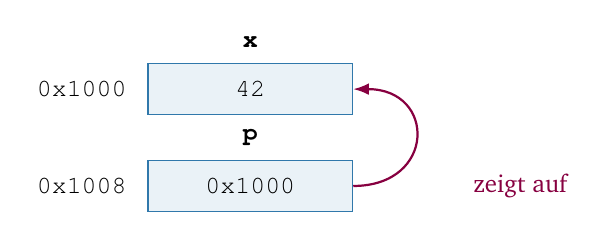
\begin{tikzpicture}[scale=0.82, every node/.style={font=\small}]
        \tikzset{membox/.style={draw=fbblau, fill=fbblau!10,
                 minimum width=2.6cm, minimum height=0.65cm,
                 font=\small\ttfamily}}
        \node[membox]           (x)  at (3, 2.5) {42};
        \node[left=4pt of x]                   {\texttt{0x1000}};
        \node[above=2pt of x, font=\bfseries\ttfamily\small] {x};

        \node[membox]           (p)  at (3, 1.0) {0x1000};
        \node[left=4pt of p]                   {\texttt{0x1008}};
        \node[above=2pt of p, font=\bfseries\ttfamily\small] {p};

        \draw[-{Latex[length=2mm]}, thick, blackberry]
          (p.east) to[out=0,in=0,looseness=2.2] (x.east);
        \node[right=1.4cm of p, color=blackberry] {zeigt auf};
      \end{tikzpicture}

      \vspace{0.4em}
      \begin{block}{Operatoren}
        \texttt{\&var} -- Adresse von \texttt{var}\\
        \texttt{*ptr} -- Wert an Adresse\\
        \texttt{ptr->feld} -- Strukturfeld via Ptr\\
        \texttt{(*ptr).feld} -- äquivalent
      \end{block}
      \begin{alertblock}{Goldene Regel}
        Pointer \emph{immer} initialisieren! \\
        Uninitialisiert = Undefined Behavior.
      \end{alertblock}
    \end{column}
  \end{columns}
\end{frame}

\begin{frame}[fragile]{Pointer-Arithmetik und Arrays}
  \begin{columns}[T]
    \begin{column}{0.52\textwidth}
\begin{lstlisting}
int arr[5] = {10, 20, 30, 40, 50};
int *p = arr;        /* = &arr[0] */

printf("%d\n", *p);      /* 10  */
printf("%d\n", *(p+1));  /* 20  */
printf("%d\n", *(p+4));  /* 50  */

p++;  /* p zeigt jetzt auf arr[1] */
printf("%d\n", *p);      /* 20  */
/* Äquivalente Schreibweisen */
arr[2]   ==  *(arr + 2)  /* true */
&arr[2]  ==  arr + 2     /* true */
/* Pointer-Differenz */
int *q   = &arr[4];
ptrdiff_t d = q - p;   /* = 3   */
/* Pointer auf Pointer */
int   x  = 5;
int  *p2 = &x;
int **pp = &p2;
**pp = 99;             /* x = 99 */
\end{lstlisting}
    \end{column}
    \begin{column}{0.45\textwidth}
      \textbf{Skalierung der Arithmetik:}
      \begin{block}{}
        \texttt{p + n} springt um \\
        $n \times \mathtt{sizeof(*p)}$ Bytes
      \end{block}

      \vspace{0.4em}
      \textbf{Array vs.\ Pointer -- wichtiger Unterschied:}
\begin{lstlisting}
int arr[5];
int *p = arr;

sizeof(arr) /* 20 Byte (5*4) */
sizeof(p)   /*  8 Byte (Ptr) */
\end{lstlisting}

      \vspace{0.2em}
      \textbf{Häufige Anwendung:}
\begin{lstlisting}
/* Iteriere mit Pointer */
uint8_t buf[8];
uint8_t *end = buf + sizeof(buf);
for (uint8_t *it = buf; it < end; it++)
    *it = 0xFF;
\end{lstlisting}
      \begin{block}{\texttt{char**argv}}
        \texttt{int main(int argc, char **argv)} --
        Pointer auf Array von Strings
      \end{block}
    \end{column}
  \end{columns}
\end{frame}

\begin{frame}[fragile]{\texttt{const}, \texttt{void*} und NULL-Pointer}
  \begin{columns}[T]
    \begin{column}{0.50\textwidth}
      \textbf{const-Qualifikation:}
\begin{lstlisting}
int x = 5;

/* Pointer auf const-Wert (read-only) */
const int *p1 = &x;
/* *p1 = 10; */    /* Fehler! */
p1 = NULL;         /* OK       */
/* Const Pointer (Adresse unveränderlich) */
int *const p2 = &x;
/* p2 = NULL; */   /* Fehler!  */
*p2 = 10;          /* OK       */
/* Beides const */
const int *const p3 = &x;
\end{lstlisting}
      \textbf{\texttt{void*} -- generischer Pointer:}
\begin{lstlisting}
void  *generic;
int    a = 42;
generic = &a;  /* kein Cast nötig */
int b = *(int*)generic; /* Cast beim Deref */

/* memcpy, memset arbeiten mit void* */
void *memcpy(void *dst,
             const void *src, size_t n);
\end{lstlisting}
    \end{column}
    \begin{column}{0.47\textwidth}
      \textbf{NULL-Pointer:}
\begin{lstlisting}
#include <stddef.h>
int *p = NULL;  /* Zeigt auf "nichts" */

if (p != NULL) {
    /* nur dann dereferenzieren! */
    printf("%d\n", *p);
}
\end{lstlisting}
      \vspace{0.3em}
      \begin{alertblock}{Sicherheitsregeln für Pointer}
        \begin{enumerate}
          \item Pointer vor Nutzung auf \texttt{NULL} prüfen
          \item Nach \texttt{free()}: \texttt{ptr = NULL} setzen
          \item Kein Pointer auf lokale (Stack-)Variable zurückgeben!
          \item Array-Grenzen \emph{immer} prüfen
          \item \texttt{const} so oft wie möglich verwenden
        \end{enumerate}
      \end{alertblock}
    \end{column}
  \end{columns}
\end{frame}

\begin{frame}[fragile]{Funktionspointer}
  \begin{columns}[T]
    \begin{column}{0.55\textwidth}
\begin{lstlisting}
/* Zwei Funktionen gleicher Signatur */
int add(int a, int b) { return a + b; }
int mul(int a, int b) { return a * b; }

/* Funktionspointer-Typ per typedef */
typedef int (*BinOp_t)(int, int);

/* Direktverwendung */
BinOp_t op = add;
printf("%d\n", op(3, 4));   /* 7  */
op = mul;
printf("%d\n", op(3, 4));   /* 12 */

/* Als Parameter (Callback-Muster) */
int apply(BinOp_t f, int x, int y) {
    return f(x, y);
}
printf("%d\n", apply(add, 10, 5)); /* 15 */

/* Dispatch-Tabelle */
BinOp_t ops[] = {add, mul};
printf("%d\n", ops[1](3, 4));     /* 12 */
\end{lstlisting}
    \end{column}
    \begin{column}{0.42\textwidth}
      \textbf{Syntax -- Merkhilfe:}
      \begin{block}{}
        \texttt{int (*fp)(int, int)}\\[0.3em]
        \small Lies: \texttt{fp} ist ein Pointer
        auf eine Funktion, die zwei \texttt{int}
        erhält und \texttt{int} zurückgibt.
      \end{block}

      \vspace{0.4em}
      \textbf{Typischer Einsatz in Embedded:}
      \begin{itemize}
        \item ISR-Registrierung und HAL-Callbacks
        \item Zustandsmaschinen als Dispatch-Tabelle
        \item Treiber-Interfaces (open/read/write/ioctl)
        \item Plugin- und Middleware-Architekturen
      \end{itemize}

      \begin{exampleblock}{Immer \texttt{typedef}!}
        Macht Funktionspointer-Typen\\
        lesbar und wartbar.
      \end{exampleblock}
    \end{column}
  \end{columns}
\end{frame}

\begin{frame}[fragile]{Typumwandlung (Casting)}
  \begin{columns}[T]
    \begin{column}{0.50\textwidth}
      \textbf{Implizite Konvertierungen:}
\begin{lstlisting}
int   i = 42;
float f = i;       /* int->float: OK   */
double d = f;      /* float->double: OK */
/* GEFÄHRLICH -- stille Kürzung! */
int    big   = 300;
uint8_t small = big;  /* 300%256 = 44! */
/* Integer Promotion: klein -> int */
uint8_t a = 200u, b = 100u;
uint8_t c = a + b; /* 300 -> 44 ! */
\end{lstlisting}
      \textbf{Expliziter Cast:}
\begin{lstlisting}
float x = 3.9f;
int   n = (int)x;  /* 3 (trunc!) */
/* Hardware-Registerzugriff */
volatile uint32_t *GPIOA =
    (volatile uint32_t *)0x40010800UL;
*GPIOA |= (1u << 5);  /* Bit 5 setzen */
\end{lstlisting}
    \end{column}
    \begin{column}{0.47\textwidth}
      \textbf{Typkonvertierungs-Hierarchie:}
      \begin{center}
        \small
        \texttt{char} $\to$ \texttt{short} $\to$ \texttt{int}
        $\to$ \texttt{long} $\to$ \texttt{float} $\to$ \texttt{double}
      \end{center}

      \vspace{0.3em}
      \textbf{Gefahrenquellen:}
\begin{lstlisting}
/* Vorzeichenwechsel */
int   neg  = -1;
uint32_t u = (uint32_t)neg; /* 2^32-1 */
/* Pointer-Aliasing (UB!) */
float  f  = 1.0f;
int   *ip = (int*)&f;  /* gefährlich */


\end{lstlisting}
      % \begin{alertblock}{Embedded-Regel}
      %   Immer explizit casten.\\
      %   Nie auf implizite Integer-Promotion verlassen!
      % \end{alertblock}
    \end{column}
  \end{columns}
\end{frame}

% ============================================================
\section{Call by Value und Speicherverwaltung}
% ============================================================

\begin{frame}[fragile]{Call by Value -- und wie wir es umgehen}
  \begin{columns}[T]
    \begin{column}{0.50\textwidth}
\begin{lstlisting}
/* C übergibt IMMER Kopien (Call by Value) */
void double_it(int x) {
    x = x * 2; /* nur lokale Kopie! */
}
int main(void) {
    int a = 5;
    double_it(a);
    printf("%d\n", a); /* Immer noch 5 */
    return 0;
}
\end{lstlisting}
      \vspace{0.3em}
\begin{lstlisting}
/* Lösung: Pointer übergeben
   ("Call by Reference" simuliert) */
void double_it_ref(int *x) {
    *x = *x * 2;
}
double_it_ref(&a);
printf("%d\n", a);    /* 10 */
/* Structs effizient übergeben */
void sensor_process(const Sensor_t *s) {
    printf("ID=%u\n", s->id);
}
\end{lstlisting}
    \end{column}
    \begin{column}{0.47\textwidth}
      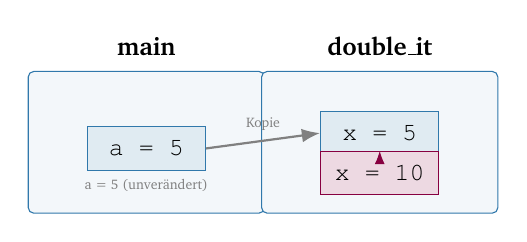
\begin{tikzpicture}[scale=0.78, every node/.style={font=\small}]
        \tikzset{
          frame/.style={draw=fbblau, fill=fbblau!6,
                        rounded corners=2pt, minimum width=3cm,
                        minimum height=1.8cm},
          var/.style={draw=fbblau, fill=fbblau!15,
                      minimum width=1.5cm, minimum height=0.55cm,
                      font=\small\ttfamily}
        }
        \node[frame] (main) at (0, 1) {};
        \node[above=2pt of main, font=\bfseries\small] {main};
        \node[var] (a)  at (0, 0.9) {a = 5};

        \node[frame] (fn)   at (3.8, 1) {};
        \node[above=2pt of fn, font=\bfseries\small] {double\_it};
        \node[var] (x1) at (3.8, 1.15) {x = 5};
        \node[var, fill=blackberry!15, draw=blackberry]
              (x2) at (3.8, 0.5) {x = 10};

        \draw[-{Latex}, thick, gray]
              (a.east) -- node[above,font=\tiny]{Kopie} (x1.west);
        \draw[-{Latex}, blackberry] (x1) -- (x2);
        \node[font=\tiny, color=gray] at (0, 0.3) {a = 5 (unverändert)};
      \end{tikzpicture}

      \vspace{0.4em}
      \begin{block}{Arrays -- immer als Pointer}
\begin{lstlisting}
/* arr zerfällt zu int* */
void zero(int *arr, size_t n){
    for (size_t i=0;i<n;i++)
        arr[i] = 0;
}
int buf[8];
zero(buf, 8);  /* keine Kopie! */
\end{lstlisting}
      \end{block}
    \end{column}
  \end{columns}
\end{frame}

\begin{frame}[fragile]{Dynamische Speicherverwaltung}
  \begin{columns}[T]
    \begin{column}{0.52\textwidth}
\begin{lstlisting}
#include <stdlib.h>
/* Heap-Allokation (uninitialisiert) */
int *arr = (int*)malloc(10 * sizeof(int));
if (arr == NULL) {
    /* Fehlerbehandlung! */
    return -1;
}
/* Calloc -- mit 0 initialisiert */
int *arr2 = (int*)calloc(10, sizeof(int));
/* Realloc -- Größe ändern */
arr = (int*)realloc(arr, 20 * sizeof(int));
if (arr == NULL) { /* ... */ }
/* Freigeben */
free(arr);
arr = NULL;   /* Dangling Pointer vermeiden */
free(arr2);
arr2 = NULL;
\end{lstlisting}
    \end{column}
    \begin{column}{0.45\textwidth}
      % \textbf{Speicherbereiche eines C-Prozesses:}
      % \vspace{0.2em}
      % \begin{center}
      %   \begin{tikzpicture}[scale=0.72]
      %     \tikzset{seg/.style={draw=fbblau, fill=fbblau!10,
      %              minimum width=3.4cm, minimum height=0.58cm,
      %              font=\small, text width=3cm, align=center}}
      %     \node[seg]                          at (0,4.2) {\textbf{Stack} (lok. Vars, Rückgabe)};
      %     \node[seg, fill=fbblau!25]          at (0,3.4) {\textbf{Heap} (malloc/free)};
      %     \node[seg, fill=gray!20]            at (0,2.6) {BSS (uninitialisierte Globals)};
      %     \node[seg, fill=gray!20]            at (0,1.8) {Data (initialisierte Globals)};
      %     \node[seg, fill=gray!40]            at (0,1.0) {Text / Code (read-only)};
      %     \draw[-{Latex}, fbblau, thick]   (-2.1,4.0) -- (-2.1,3.7)
      %           node[right, font=\tiny] {$\downarrow$ wächst};
      %     \draw[-{Latex}, fbblau!60, thick] (-2.1,3.0) -- (-2.1,3.2)
      %           node[right, font=\tiny] {$\uparrow$ wächst};
      %   \end{tikzpicture}
      % \end{center}
      \begin{alertblock}{Embedded-Empfehlung}
        In sicherheitskritischen und Echtzeitsystemen \texttt{malloc} nach Möglichkeit \emph{vermeiden} -- statische oder
        Stack-Allokation bevorzugen (MISRA-C Regel).
      \end{alertblock}
    \end{column}
  \end{columns}
\end{frame}

% ============================================================
\section{Objektorientierung in C simulieren}
% ============================================================

\begin{frame}[fragile]{Structs als Klassen -- das \texttt{self}-Muster}
  \begin{columns}[T]
    \begin{column}{0.52\textwidth}
\begin{lstlisting}
#include <math.h>
/* "Klasse" = Struct als Datenkapsel */
typedef struct {
    float x, y;
} Point_t;
/* "Methoden" = Funktionen mit self-Ptr
   (analog zu C++ this-Pointer)       */
void Point_init(Point_t *self,
                float x, float y) {
    self->x = x;
    self->y = y;
}
float Point_dist(const Point_t *self,
                 const Point_t *other) {
    float dx = self->x - other->x;
    float dy = self->y - other->y;
    return sqrtf(dx*dx + dy*dy);
}
/* Verwendung */
Point_t p1, p2;
Point_init(&p1, 0.0f, 0.0f);
Point_init(&p2, 3.0f, 4.0f);
float d = Point_dist(&p1, &p2); /* 5.0 */
\end{lstlisting}
    \end{column}
    \begin{column}{0.45\textwidth}
      \textbf{Namenskonventionen:}
      \begin{itemize}
        \item Typ: \texttt{TypeName\_t}
        \item Konstruktor: \texttt{TypeName\_init()} \\
              bzw.\ \texttt{TypeName\_create()}
        \item Methoden: \texttt{TypeName\_verb()}
        \item Erster Parameter immer \texttt{self}
        \item \texttt{const} für lesende Methoden
      \end{itemize}
      \vspace{0.3em}
      \begin{block}{Kapselung durch Header-Trennung}
        \textbf{point.h} -- öffentliche API:\\
        \texttt{typedef} + Prototypen\\[0.3em]
        \textbf{point.c} -- Implementierung:\\
        Struct-Felder + Funktionskörper\\[0.3em]
        $\Rightarrow$ Nutzer sieht \emph{nur} das Interface
      \end{block}
      \begin{exampleblock}{Analogie C++ $\leftrightarrow$ C}
        \texttt{class} $\leftrightarrow$ \texttt{struct}\\
        \texttt{this} $\leftrightarrow$ \texttt{self}\\
        Methode $\leftrightarrow$ Funktion + \texttt{self}-Ptr
      \end{exampleblock}
    \end{column}
  \end{columns}
\end{frame}

\begin{frame}[fragile]{Polymorphismus mit Funktionspointern (vtable)}
  \begin{columns}[T]
    \begin{column}{0.55\textwidth}
\begin{lstlisting}
/* Vorwärtsdeklaration */
typedef struct Shape_s Shape_t;
/* Virtuelle Methodentabelle */
typedef float (*AreaFn_t)(const Shape_t *);
typedef void  (*DrawFn_t)(const Shape_t *);
typedef struct {
    AreaFn_t  area;
    DrawFn_t  draw;
} ShapeVTable_t;
/* Basisklasse */
struct Shape_s {
    const ShapeVTable_t *vtable;
    float x, y;
};
/* Abgeleitete "Klasse" */
typedef struct {
    Shape_t base;   /* Vererbung: zuerst! */
    float   radius;
} Circle_t;
float Circle_area(const Shape_t *self) {
    const Circle_t *c = (const Circle_t*)self;
    return 3.14159f * c->radius * c->radius;
}
void Circle_draw(const Shape_t *self) {
    printf("Circle r=%.1f\n",
           ((const Circle_t*)self)->radius);
}
\end{lstlisting}
    \end{column}
    \begin{column}{0.42\textwidth}
\begin{lstlisting}
static const ShapeVTable_t
  circle_vtable = {
    .area = Circle_area,
    .draw = Circle_draw
};
void Circle_init(Circle_t *c,
    float x, float y, float r) {
    c->base.vtable = &circle_vtable;
    c->base.x = x;
    c->base.y = y;
    c->radius = r;
}
/* Polymorpher Aufruf */
Circle_t circ;
Circle_init(&circ, 0,0, 5.0f);

Shape_t *s = (Shape_t*)&circ;
s->vtable->area(s);  /* dispatch! */
s->vtable->draw(s);
\end{lstlisting}
      \begin{block}{Vererbung in C}
        Abgeleitetes Struct enthält\\
        Basisstruct als \emph{erstes} Member.\\
        Cast zu Basistyp ist dann sicher.
      \end{block}
    \end{column}
  \end{columns}
\end{frame}

\begin{frame}[fragile]{Kapselung mit Opaque Pointer}
  \begin{columns}[T]
    \begin{column}{0.50\textwidth}
      \textbf{Öffentlicher Header \texttt{sensor.h}:}
\begin{lstlisting}
#ifndef SENSOR_H
#define SENSOR_H
#include <stdint.h>

/* Opaque Pointer -- Nutzer kennt nur   den Typ, nicht die Felder!    */
typedef struct Sensor_s Sensor_t;

/* Konstruktor und Destruktor */
Sensor_t *Sensor_create(uint8_t id);
void      Sensor_destroy(Sensor_t *self);

/* Öffentliche Methoden */
float Sensor_read(Sensor_t *self);
void  Sensor_calibrate(Sensor_t *self,
                       float offset);
float Sensor_last(const Sensor_t *self);

#endif /* SENSOR_H */
\end{lstlisting}
    \end{column}
    \begin{column}{0.47\textwidth}
      \textbf{Implementierung \texttt{sensor.c}:}
\begin{lstlisting}
#include "sensor.h"
#include <stdlib.h>

/* Struct-Definition: nur HIER sichtbar */
struct Sensor_s {
    uint8_t  id;
    float    offset;
    float    last_value;
};

Sensor_t *Sensor_create(uint8_t id) {
    Sensor_t *s = malloc(sizeof(*s));
    if (s != NULL) {
        s->id         = id;
        s->offset     = 0.0f;
        s->last_value = 0.0f;
    }
    return s;
}

void Sensor_destroy(Sensor_t *self) {
    free(self);
}

float Sensor_read(Sensor_t *self) {
    /* Hardware-Zugriff (Platzhalter) */
    self->last_value = read_hw_adc(self->id)
                       + self->offset;
    return self->last_value;
}
\end{lstlisting}
    \end{column}
  \end{columns}
\end{frame}

% ============================================================
\section{Zusammenfassung}
% ============================================================

\begin{frame}{Zusammenfassung}
  \begin{columns}[T]
    \begin{column}{0.48\textwidth}
      \textbf{Geschichte \& Standards:}
      \begin{itemize}
        \item C seit 1972 (Ritchie, Bell Labs, Unix)
        \item Standards: C89 $\to$ C99 $\to$ C11 $\to$ C17 $\to$ C23
        \item Ideal für Embedded: Hardwarenähe, Effizienz, Deterministismus
      \end{itemize}
      \textbf{Grundkonstrukte:}
      \begin{itemize}
        \item Portable Typen (\texttt{stdint.h}) bevorzugen
        \item \texttt{struct}, \texttt{enum}, \texttt{typedef} für Abstraktion
        \item \texttt{volatile} für Hardware-Register unverzichtbar
        \item \texttt{static} für Datenkapselung auf Dateiebene
      \end{itemize}
    \end{column}
    \begin{column}{0.48\textwidth}
      \textbf{Zeiger und Typsystem:}
      \begin{itemize}
        \item \texttt{\&} / \texttt{*}: Adresse und Dereferenzierung
        \item Pointer-Arithmetik skaliert mit \texttt{sizeof}
        \item Funktionspointer für Callbacks und Dispatch-Tabellen
        \item Casts immer explizit; \texttt{void*} für Generizität
        \item \texttt{const} so früh und so oft wie möglich
      \end{itemize}
      \textbf{OOP-Muster in C:}
      \begin{itemize}
        \item \texttt{struct} als Klasse, \texttt{self}-Pointer als \texttt{this}
        \item Funktionspointer im Struct $\to$ vtable $\to$ Polymorphismus
        \item Opaque Pointer $\to$ echte Kapselung
        \item Call by Reference: Pointer übergeben
      \end{itemize}
    \end{column}
  \end{columns}

  \vspace{0.6em}
  \begin{center}
    \large\color{fbblau}\rule{0.4\textwidth}{0.4pt}\quad
    \textbf{Fragen?}
    \quad\rule{0.4\textwidth}{0.4pt}
  \end{center}
\end{frame}

% ============================================================
\end{document}
